%%%%%%%%%%%%%%%%%%%%%%%%%%%%%%%%%%%%%%%%%
% fphw Assignment
% LaTeX Template
% Version 1.0 (27/04/2019)
%
% This template originates from:
% https://www.LaTeXTemplates.com
%
% Authors:
% Class by Felipe Portales-Oliva (f.portales.oliva@gmail.com) with template 
% content and modifications by Vel (vel@LaTeXTemplates.com)
%
% Template (this file) License:
% CC BY-NC-SA 3.0 (http://creativecommons.org/licenses/by-nc-sa/3.0/)
%
%%%%%%%%%%%%%%%%%%%%%%%%%%%%%%%%%%%%%%%%%

%----------------------------------------------------------------------------------------
%	PACKAGES AND OTHER DOCUMENT CONFIGURATIONS
%----------------------------------------------------------------------------------------

\documentclass[
	12pt, % Default font size, values between 10pt-12pt are allowed
	%letterpaper, % Uncomment for US letter paper size
	%spanish, % Uncomment for Spanish
]{fphw}

% Template-specific packages
\usepackage[utf8]{inputenc} % Required for inputting international characters
\usepackage[T1]{fontenc} % Output font encoding for international characters
\usepackage{mathpazo} % Use the Palatino font
\usepackage[dvipsnames]{xcolor}
\usepackage{graphicx} % Required for including images
\usepackage{amsmath}
\usepackage{booktabs} % Required for better horizontal rules in tables
\usepackage{listings} % Required for insertion of code
\usepackage{enumerate} % To modify the enumerate environment
\usepackage{ragged2e}
\usepackage{cancel}
\usepackage{MnSymbol,bbding,pifont}
\usepackage{lscape}
\usepackage{array}
\usepackage{float,graphicx}
\usepackage{hyperref}
\newcolumntype{M}{>{$}c<{$}}
%----------------------------------------------------------------------------------------
%	ASSIGNMENT INFORMATION
%----------------------------------------------------------------------------------------

\title{Assignment \#1} % Assignment title

\author{Luis Alberto Ballado Aradias} % Student name

\date{\today} % Due date

\institute{Centro de Investigación y de Estudios Avanzados del IPN \\ Unidad Tamaulipas} % Institute or school name

\class{CONTROL AUTOMÁTICO (Sep - Dec 2022)} % Course or class name

\professor{Dr. José Gabriel Ramírez Torres} % Professor or teacher in charge of the assignment

%----------------------------------------------------------------------------------------

\begin{document}

\maketitle % Output the assignment title, created automatically using the information in the custom commands above

%----------------------------------------------------------------------------------------
%	ASSIGNMENT CONTENT
%----------------------------------------------------------------------------------------
\section*{{\color{Apricot}Climate-neutral container terminal: How does it work?} \url{https://www.youtube.com/watch?v=wiKS-RYf-cY}}

La automatización en puertos maritimos ha tomado un auge de la mano con la industria 4.0 y la era del internet, la automatización como el uso de energia verdes nos comienza a acompañar a donde sea que vayamos. La globalización se ha convertido en una tendencia en la economía global y los sistemas de control automáticos son una pieza clave.\\

\begin{figure}[H]
  \centering
  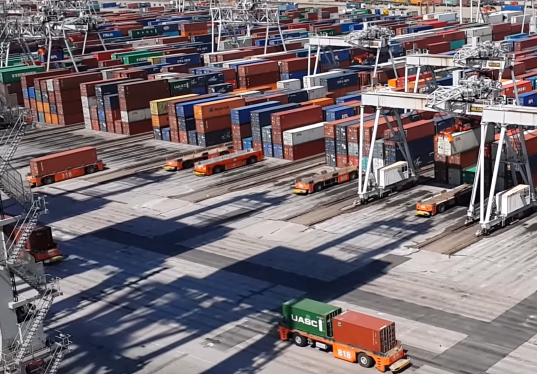
\includegraphics[scale=0.4]{images/puerto.png}
\end{figure}

Según los datos de las \href{https://news.un.org/es/story/2021/11/1500122}{Naciones Unidas} el embate provocado por la pandemia de COVID-19 sobre el transporte maritimo de mercancias tuvo menos repercusión ya que la demanda global ocacionada por las compras electrónicas ayudo en generar un aumento del 4,3\% en 2021. \\

Para cualquier empresa donde las tareas se convierten en repetitivas y aburridas, es de buena opción automatizar dichos procesos cuando estos sean tecnológicamente posibles, ya que tareas comunes como cocinar, hacer una limpieza en áreas con muchos objetos suelen ser dificiles de automatizar.\\

\begin{figure}[H]
  \centering
  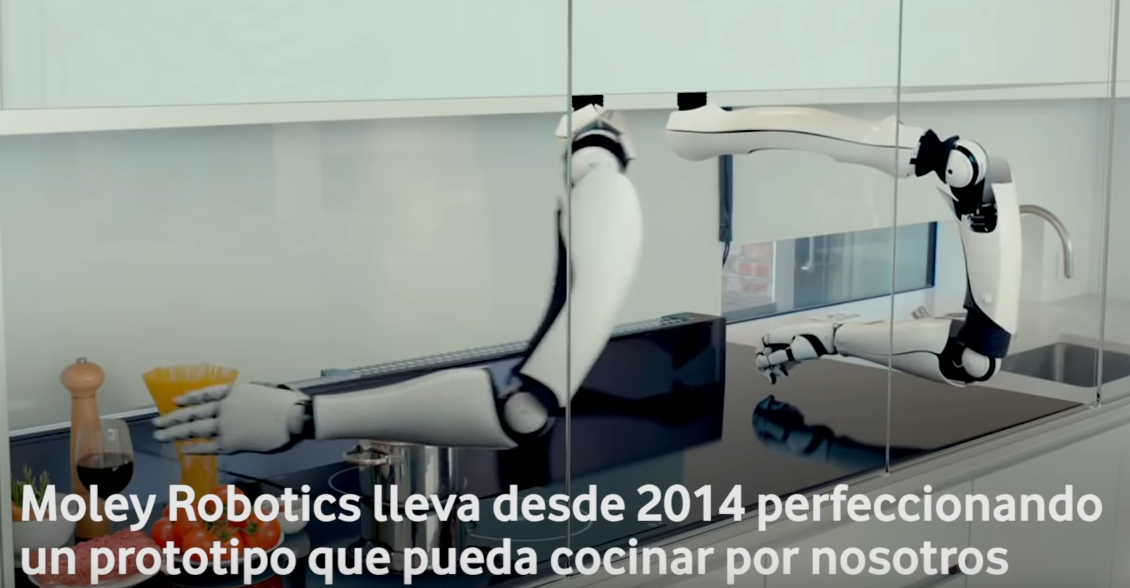
\includegraphics[scale=0.4]{images/hard.png}
\end{figure}

El futuro de la logistica, transporte marítimo ó terrestre tiene un futuro inteligente y sostenible. Teniendo ejemplos tangibles en los Puertos de Hamburgo, Shangai, Rotterdam por mencionar algunos.\\

La implementacion de vehículos AGV (Automated Guided Vehicles) en la industria de la logistica ha tomado un gran auge, no es dificil pensar que el grande de las ventas por internet AMAZON tenga una implementación en sus centros de distribución de ultima milla casi todo automatizado.\\

Para su construcción, mantenimiento, y desarrollo de sistemas inteligentes es de suma importancia el estudio de Sistemas de Control.

\begin{figure}[H]
  \centering
  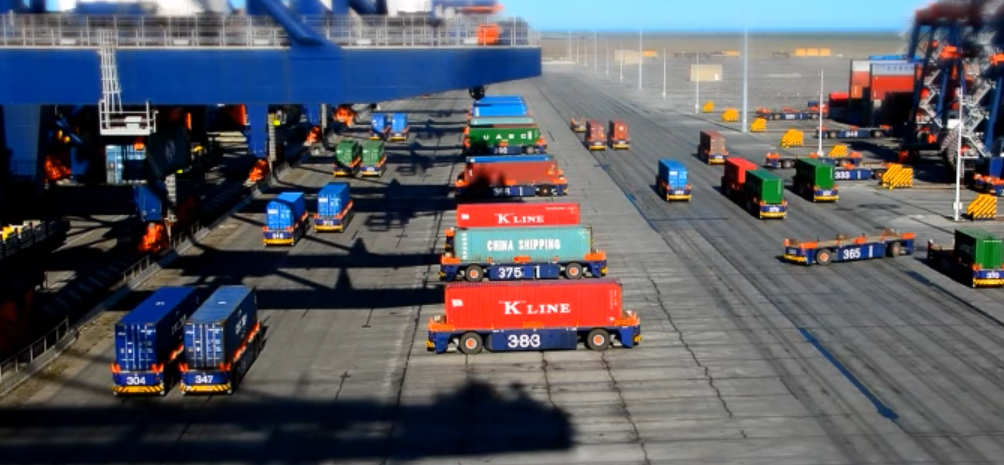
\includegraphics[scale=0.4]{images/agv.png}
\end{figure}

\newpage
\section*{{\color{Apricot}Why learn control systems at all?} \url{https://www.youtube.com/watch?v=oBc_BHxw78s}}

Los sistemas de control es la pieza que une todos los campos de la ingenieria.\\

Considerando algunos campos de la ingenieria podemos entender un poco más la importancia en el estudio del Control automático.

\begin{itemize}
\item Ingenieria Eléctica, en el diseño de reguladores y retroalimentaciones inestables
\item Ingenieria en Comunicaciones, en el diseño de controles de ganancia automáticas que incrementen la ganancia en señales débiles o decrementarlas en señales fuertes.
\item Ingeniera Mecánica, en la consideración de vibraciones, diseño de sistemas que aislen las vibraciones. 
\item Ingeniera Civil, en el diseño de construcciones resistentes a actividades sismicas.
\item Ingeniera Industrial, en el diseño de robótica para lineas de ensamblaje o diseño de controles para aplicaciones en la robótica.
\item Ingeniera Aeroespacial, en la creación de sistemas aerodinamicos resistentes a las vibraciones.
\end{itemize}

Una perspectiva general de los sistemas de control sería cuando se nos cae un objeto, éste vibrará y generará un sonido que se reducira a medida que la energía se disipe, o cuando intentamos detener una caida de algun objeto y causamos una disipasión rápida de la energía. \\

Detrás de la tecnologia de un giroscopio que es ((DECIR QUE ES)) y es usado en submarinos, satelites 

\newpage
\section*{{\color{Cerulean} Automation} \url{https://www.youtube.com/watch?v=XJLMW6l303g}}

\begin{figure}[H]
  \centering
  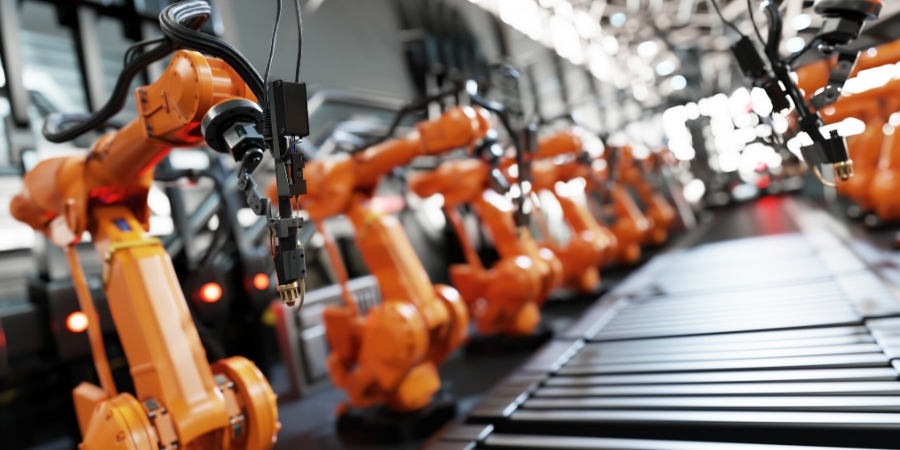
\includegraphics[scale=0.3]{images/automation.jpg}
\end{figure}

\newpage
\section*{{\color{RoyalPurple}Tacoma Bridge} \url{https://www.youtube.com/watch?v=3mclp9QmCGs}}

\begin{figure}[H]
  \centering
  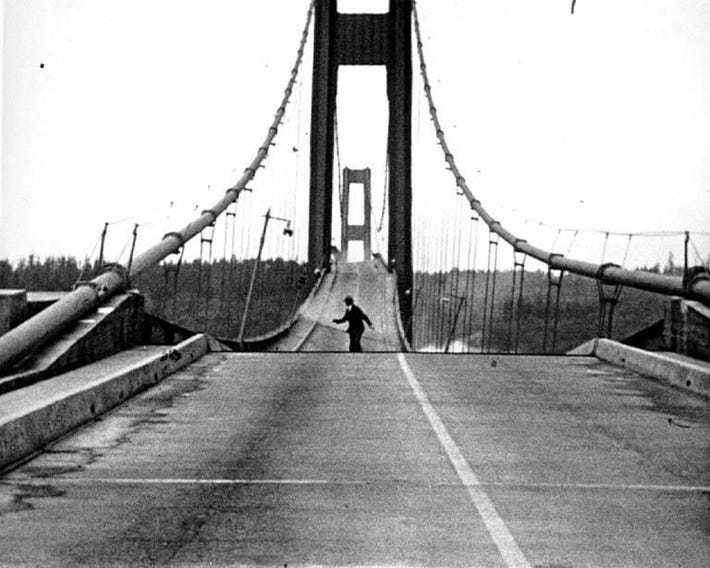
\includegraphics[scale=0.3]{images/tacoma.jpg}
\end{figure}

\newpage
\section*{{\color{RoyalPurple}What Control Systems Engineers Do?} \url{https://www.youtube.com/watch?v=ApMz1-MK9IQ}}

\begin{figure}[H]
  \centering
  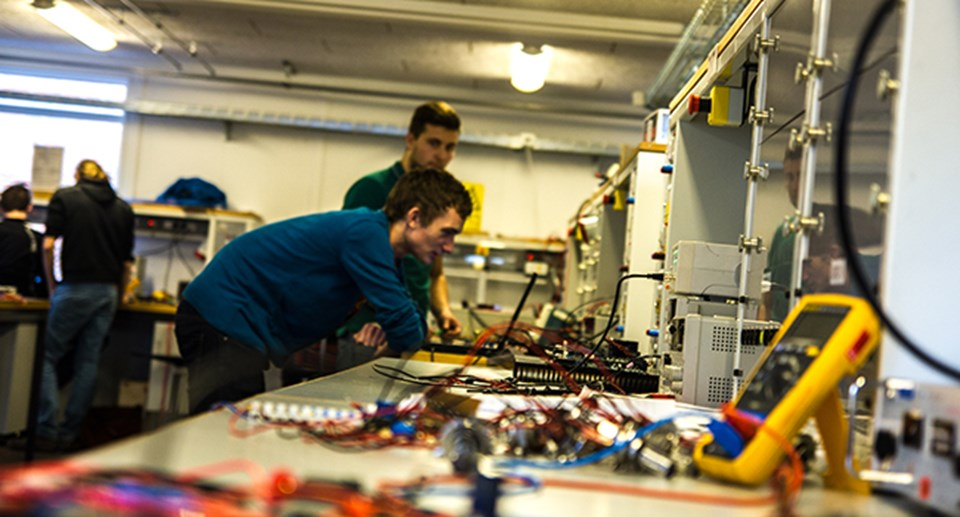
\includegraphics[scale=0.3]{images/control_ing.jpg}
\end{figure}

\newpage
\section*{{\color{RoyalPurple}Control Systems Lectures LTI Systems} \url{https://www.youtube.com/watch?v=3eDDTFcSC_Y}}

\begin{figure}[H]
  \centering
  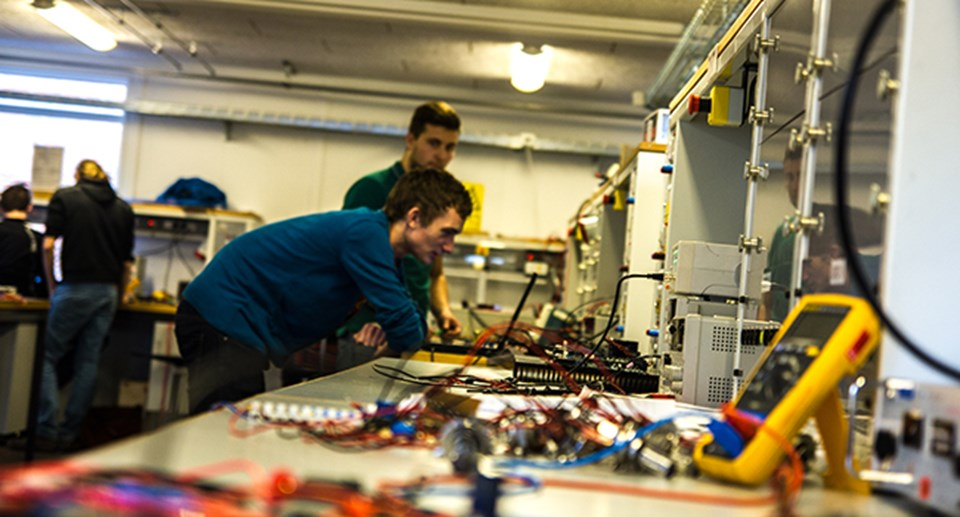
\includegraphics[scale=0.3]{images/control_ing.jpg}
\end{figure}

\newpage
\section*{{\color{RoyalPurple}Laplace transform} \url{https://www.youtube.com/watch?v=VJ9phDRys_I}}

\begin{figure}[H]
  \centering
  \includegraphics[scale=0.3]{images/}
\end{figure}

\newpage
\section*{{\color{RoyalPurple}Transfer functions} \url{https://www.youtube.com/watch?v=RJleGwXorUk}}

\begin{figure}[H]
  \centering
  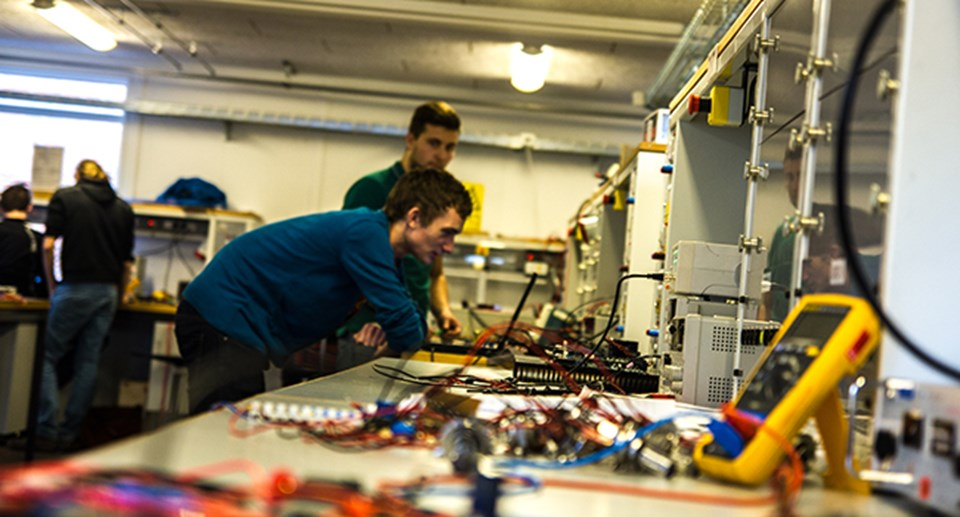
\includegraphics[scale=0.3]{images/control_ing.jpg}
\end{figure}

\end{document}
